\documentclass{article}
\title{Janim Example 2}
\author{John Doe}
\usepackage{tikz}
\usepackage{geometry}
\geometry{
paperheight=216mm,paperwidth=384mm,
total={344mm,176mm},
left=20mm,
top=20mm,
}
\usepackage{fontspec}
\usepackage{xcolor}
\setmainfont{CascadiaMono.ttf}
\pagenumbering{gobble}
\pagecolor{white}
\hyphenpenalty 10000
\exhyphenpenalty 10000
\begin{document}
\maketitle
\noindent \textcolor{black}
{\Huge \textcolor{blue}{Finite Automata}}
\noindent \textcolor{black}
{\vspace{5mm}}
\noindent \textcolor{black}
{\textbf{Example 1: DFA for strings ending with 'a'}}
\noindent \textcolor{black}
{\vspace{2mm}}
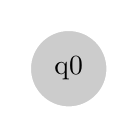
\begin{tikzpicture}
\filldraw[color=white!60, fill=black!20, very thick](10mm,10mm) circle (5mm);
\node at (10mm,10mm) {q0};
\end{tikzpicture}

\begin{tikzpicture}
\filldraw[color=white!60, fill=black!20, very thick](10mm,10mm) circle (5mm);
\node at (10mm,10mm) {};
\end{tikzpicture}
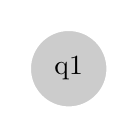
\begin{tikzpicture}
\filldraw[color=white!60, fill=black!20, very thick](10mm,10mm) circle (5mm);
\node at (10mm,10mm) {q1};
\end{tikzpicture}

\begin{tikzpicture}
\filldraw[color=white!60, fill=black!20, very thick](10mm,10mm) circle (5mm);
\filldraw[color=white!60, fill=none, very thick](10mm,10mm) circle (4mm);
\node at (10mm,10mm) {};
\end{tikzpicture}
\noindent \textcolor{black}
{\vspace{30mm}}
\noindent \textcolor{black}
{\textbf{Example 2: NFA for strings containing 'aa' or 'bb'}}
\noindent \textcolor{black}
{\vspace{2mm}}
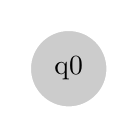
\begin{tikzpicture}
\filldraw[color=white!60, fill=black!20, very thick](10mm,10mm) circle (5mm);
\node at (10mm,10mm) {q0};
\end{tikzpicture}

\begin{tikzpicture}
\filldraw[color=white!60, fill=black!20, very thick](10mm,10mm) circle (5mm);
\node at (10mm,10mm) {};
\end{tikzpicture}
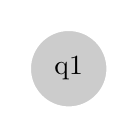
\begin{tikzpicture}
\filldraw[color=white!60, fill=black!20, very thick](10mm,10mm) circle (5mm);
\node at (10mm,10mm) {q1};
\end{tikzpicture}

\begin{tikzpicture}
\filldraw[color=white!60, fill=black!20, very thick](10mm,10mm) circle (5mm);
\filldraw[color=white!60, fill=none, very thick](10mm,10mm) circle (4mm);
\node at (10mm,10mm) {};
\end{tikzpicture}
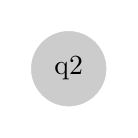
\begin{tikzpicture}
\filldraw[color=white!60, fill=black!20, very thick](10mm,10mm) circle (5mm);
\node at (10mm,10mm) {q2};
\end{tikzpicture}
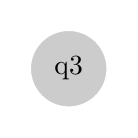
\begin{tikzpicture}
\filldraw[color=white!60, fill=black!20, very thick](10mm,10mm) circle (5mm);
\node at (10mm,10mm) {q3};
\end{tikzpicture}

\begin{tikzpicture}
\filldraw[color=white!60, fill=black!20, very thick](10mm,10mm) circle (5mm);
\filldraw[color=white!60, fill=none, very thick](10mm,10mm) circle (4mm);
\node at (10mm,10mm) {};
\end{tikzpicture}
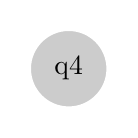
\begin{tikzpicture}
\filldraw[color=white!60, fill=black!20, very thick](10mm,10mm) circle (5mm);
\node at (10mm,10mm) {q4};
\end{tikzpicture}
\noindent \textcolor{black}
{\vspace{20mm}}
\noindent \textcolor{black}
{\textcolor{black}{This document shows two finite automata examples:}}
\noindent \textcolor{black}
{\begin{itemize}}
\noindent \textcolor{black}
{\item A DFA that accepts all strings over {a,b} ending with 'a'}
\noindent \textcolor{black}
{\item An NFA that accepts strings containing 'aa' or 'bb' as a substring}
\noindent \textcolor{black}
{\end{itemize}}
\end{document}
